\section{Design}

In this section we describe our design for a fully
disaggregated lock-based cuckoo hash. First we describe a
new dependent hashing algorithm that increases the
probability that two cuckoo hash locations will be near one
another. Using this locality we describe a new locking
scheme designed for RDMA NICs which exploits row locality to
reduce the round trips required for lock acquisition. Next
we describe a locality aware search algorithm (A*) which
produces short insertion paths in the cuckoo hash. Finally
we outline a protocol for insert, read, update and delete to
the cuckoo hash which uses our locking and search schemes.

\label{sec:design}

\begin{figure*}[t]
    \centering
    \begin{subfigure}{0.3\linewidth}
        \begin{align*}
            L_1 &= h_1(k) \\
            L_2 &= L_1 + (h_2(k)\mod f^{f + log_2(h_3(k))})
        \end{align*}
        % \caption{}
        % \label{fig:hash_factor}
    \end{subfigure}
    \begin{subfigure}{0.3\linewidth}
        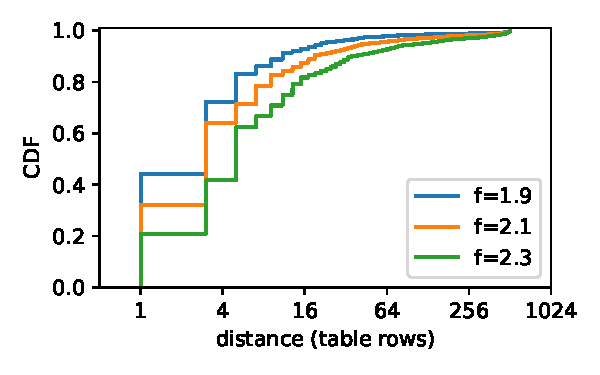
\includegraphics[width=0.99\linewidth]{fig/hash_factor.pdf}
        % \label{fig:hash_factor}
        % \caption{}
    \end{subfigure}
    \begin{subfigure}{0.3\linewidth}
        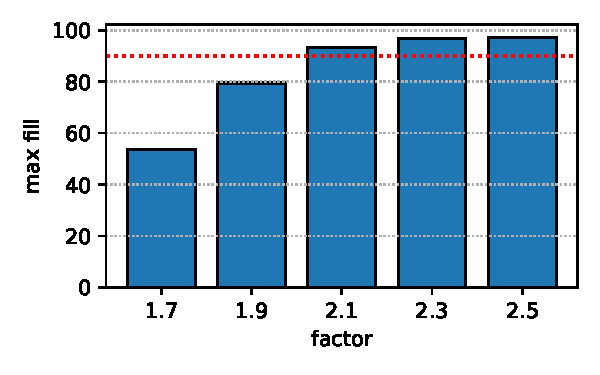
\includegraphics[width=0.99\linewidth]{fig/hash_fill.pdf}
        % \label{fig:hash_fill}
        % \caption{}
    \end{subfigure}.
    \vspace{-1em}
    \caption{
    \textbf{(a)} Dependent hashing for factor $f$.
    \textbf{(b)} CDF of distances between cuckoo locations dependent hashing on different exponential factors.
    \textbf{(c)} Exponential factor relation to max fill in cuckoo hash.
    }
    \label{fig:locality-hashing}

\end{figure*}




\subsection{Dependent Hashing}

Cuckoo and hopscotch hashes are optimized for
reads~\cite{cuckoo,hopscotch} and have been used extensively
in RDMA key value
stores~\cite{memc3,cuckoo-improvements,pilaf,farm}. Both
hashes are read optimized, cuckoo hashing ensures at most
two reads are required (both can be done in parallel), while
hopscotch hashing ensures the locality of a read to a
specific location.

Our approach aims to combine the constant time reads of
cuckoo hashing with the locality properties of hopscotch
hashing. Cuckoo hashing calls for two independent hash
functions for each key, we instead use two
~\textit{dependent} hash functions to increase locality. The
first hash function selects a row in the cuckoo table
uniformly at random. The second second hash function selects
a location randomly from the following $n$ rows after the
first hash. That is the second location will be within $n$
rows of the first hash location. The value of $n$ is not
constant. Instead we use a third hash function to generate
values of $n$ according to an exponential distribution. We
use a constant factor $f$ to control the exponential
function.  Figure~\ref{fig:locality-hashing}(a) shows the
formula for our dependent hash functions.

Small values of $f$ increase the locality of the second
function.  Figure~\ref{fig:locality-hashing}(b) illustrates
how increasing the exponential factor shifts the
distribution of distances between cuckoo hash locations.

Adding locality to the second hash function is not free.
Independence between hash functions reduces the probability
of hot spots. An over filled reigon of the table can quickly
lead to deadlocks when inserting requiring the table to be
resized. $f$ is directly related to the max fill factor of
the table. Larger $f$ values increase the max fill factor,
while decreasing locality.
Figure~\ref{fig:locality-hashing}(c) shows how these same
factors effect the max fill rate of the table before an item
cannot be inserted. The associativity of the cuckoo hash
plays a key role in enabling high fill. The higher the
degree of associativity the greater degrees of freedom
search is given to escape local hotspots.

%The second hash function determines the maximum
%distance the second value can have from the first. A third
%hash function determines a random location between the first
%location, and the bound imposed by the second.
% Figure~\ref{fig:locality-hashing}(a) shows the formula for our hashing
% function process, which implements the probabilistic region-size
% selection with a third hash function---akin to the way Bitcoin
% computes its difficulty.
% \textbf{Why not make the second hash function a true expoential?}

% A strawman implementation of locality based hashing would
% use the first hash function to find a location, and the
% second to find a random location within a fixed bound. This
% approach quickly leads to failed insertions. Due to the
% birthday paradox the probability of a collision is high, and
% on large tables the probability that one region of the hash
% table will become full, and have not viable path to an open
% slot is high. ~\sg{Perhaps this justifies a figure, please
% advise.}.

% We use a dynamic exponential bound rather than a static one.
% The dynamic bound is set by raising a constant factor $f$ by
% an exponent determined by a third hash function. Using the
% third hash on the key we count the number of suffix zeros
% and raise the constant factor by itself plus the zero count.
% This distribution generates exponential distances between
% hash locations at exponentially less frequency and is
% tunable with the single parameter $f$.
% %%
% In the common case the bound is small. Exponentially few key
% are spaced far apart and act as~\textit{waypoints} to other
% regions of the table when constructing cuckoo paths. This
% method, paired with bucket associativity enables high fill
% rates while keeping the region of the table any given key
% can inhabit small.

% There is a tradeoff between locality and fill factor.
% Figure~\ref{fig:locality-hashing}(b) illustrates how
% increasing the exponential factor shifts the distribution of
% distances between cuckoo hash locations.
% Figure~\ref{fig:locality-hashing}(c) shows how these same
% factors effect the max fill rate of the table before an item
% cannot be inserted. As will be shown in the following
% sections read, and insert performance improve with better
% locality. Therefore fill factor and performance can be
% traded off directly by changing the exponential factor. In
% our evaluation we found an exponential factor of 2.3 to give
% the best results in terms of end to end performance and
% bandwidth consumption.


\subsection{Locking}

\begin{figure*}[t]
    \centering
    \begin{subfigure}{0.3\linewidth}
        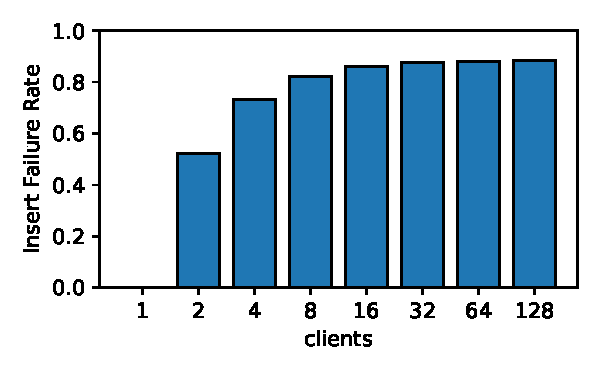
\includegraphics[width=0.99\linewidth]{fig/optimistic_failures.pdf}
        % \label{fig:optimistic_failures}
        % \caption{}
    \end{subfigure}
    \begin{subfigure}{0.3\linewidth}
        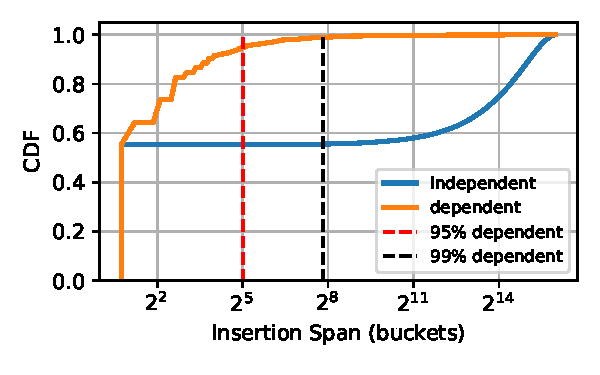
\includegraphics[width=0.99\linewidth]{fig/insertion_span.pdf}
        \label{fig:insertion_span}
        % \caption{}
    \end{subfigure}.
    \begin{subfigure}{0.3\linewidth}
        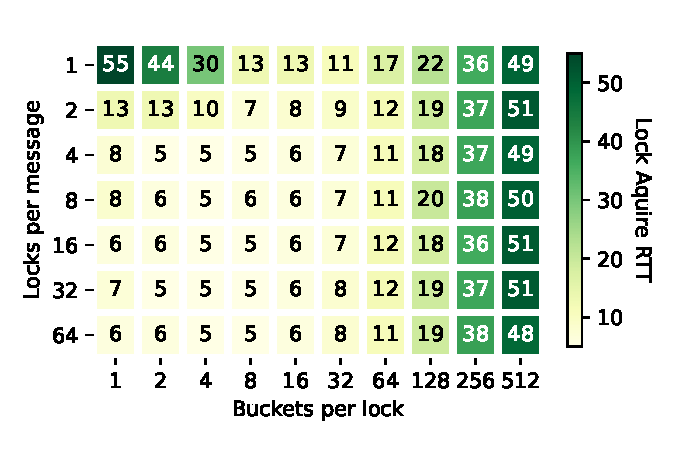
\includegraphics[width=0.99\linewidth]{fig/buckets_per_lock_vs_locks_per_message.pdf}
        \label{fig:tbd}
        % \caption{}
    \end{subfigure}.
    \vspace{-1em}
    \caption{
    \textbf{(a)} Failure rate of optimistic cuckoo insertions.
    \textbf{(b)} CDF of cuckoo spans for dependent and independent hashing. A cuckoo span is the distance between the smallest and largest index in a cuckoo path.
    \textbf{(c)} Round trips (99th percentile) required per insert while filling a table to 100\% while varying the lock per message, and buckets per lock. \todo{subtract one from each current values include unlocks}
    }
    \label{fig:cuckoo-problems}

\end{figure*}

To guard access to the table when performing modifications
we use locks. Our lock table is an array of contiguous bits
where each bit is a lock, and each lock guards one or more
sequential buckets.

We use RDMA device memory for our lock table. To aquire
locks clients locally determine which locks they require for
their operation, and then issue RDMA masked CAS operations
to the device memory. This approach enable clients to aquire
up to 64 contiguous locks with a single RDMA operation and
enable clients to aquire locks without synchronizing the
state of the lock table prior to acquisition (non masked CAS
would need the state of all locks prior to issuing the
request.).

Using this locking scheme locality hashing greatly improves
locking performance. With independent hashing the locks for
a cuckoo path are scattered randomly throughout the table.
Therefore, a round trip is required for each lock, and each
lock must be acquired in order to avoid deadlock. With
locality, and the ability to lock up to 64 sequential locks
most insertions can be performed with a single round trip
for locking. In both cases lock release can be batched in a
single round trip.

Figure~\ref{fig:cuckoo-problems}(b) shows the insert span in
buckets using both dependent and independent hashing on a
table with 500K entries and an associativity of 8. A span is
calculated as the distance between the lowest index and the
highest index in a cuckoo path. Past 50\% independent
hashing spans a random range in the table (whenever a
displacement occurs on insert). With dependent locality
based hashing 95\% of inserts span less than 32 buckets, and
99\% less than 256.


% Traditional wisdom would suggest that because cuckoo hashing
% can have long insertion paths it is a poor candidate for
% remote memory. Both opportunistic, and lock based approaches
% have significant drawbacks.
% %%
% As an example consider an opportunistic approach in which
% many clients are inserting concurrently to a table. Clients
% making inserts first make reads of the table to locally
% calculate a cuckoo path for their insertion. After the reads
% complete the client constructs a cuckoo path and starting
% from the open slot issues dependent CAS requests migrating
% the open slot backwards to the insertion bucket.
% %%
% Figure~\ref{fig:cuckoo-problems}(a) shows the failure rate
% of this insertion scheme as a factor of clients running
% inserts on a table with 500K entries with a bucket
% associativity 8. Cuckoo paths calculated from client caches
% quickly become invalid as the number of clients grows.
% %%
% Alternatively deadlock free lock acquisition requires more
% round trips and has larger critical sections. Each lock must
% be acquired in order with a dependent CAS request which
% incurs an additional round trip per lock. Using course
% grained locks reduces the number of acquisitions but
% throttles throughput as concurrent insertions are more
% likely to contend shared locks.

% Locality hashing increases the probability that an insertion
% path is within a small region of the hash table which in
% turn increases the probability that fine grained locks will
% be near one another. 
% %%
% Figure~\ref{fig:cuckoo-problems}(b) shows the insert span in
% buckets using both dependent and independent hashing on a
% table with 500K entries and an associativity of 8. A span is
% calculated as the distance between the lowest index and the
% highest index in a cuckoo path. Past 50\% independent
% hashing spans a random range in the table (whenever a
% displacement occurs on insert). With dependent locality
% based hashing 95\% of inserts span less than 32 buckets, and
% 99\% less than 256.
% %%
% RDMA masked CAS operations allow a client to set a 64 bit
% mask along with the new, and old values of the cas
% operation. So locks can be acquired with minimal knowledge
% of the remote lock table. This enables the client to
% atomically set up to 64 contiguous locks independently which
% dramatically reduces the round trips required to aquire
% locks.

% Lock granularity effects performance under contention. Using
% values from Figure~\ref{fig:cuckoo-problems}(b) if locks are
% per bucket 96\% of lock acquisitions can be completed with a
% single RTT masked cas. If locks span 4 buckets 99\% of
% requests can be completed in a single round trip.

% Increasing the number of buckets each lock guards can reduce
% the number of locks required for an operation.
% Figure~\ref{fig:ycsb_fill_latency}(c) shows the tradeoff
% between lock granularity and the number of locks which can
% be set in a single message with locality hashing turned on.
% The table has 512 rows total to illustrate the effect of a
% single global lock.

% The values
% reported are the 99th percentile number of round trips
% required to acquire locks up to a 90\% fill factor on a
% table with 4096 entries and 8 entries per bucket, and 8
% concurrent clients. The biggest factor in round trip times
% is the number of locks per bucket. On the far right side of
% the heatmap (512) only a single global lock exists. Further
% the benefit in terms of locks per message falls off quickly
% after two. RDMA-masked CAS are beneficial as they allow for
% fine-grained locking, but setting 3 or more locks per
% message has little effect up to 90\% fill rate. Reducing
% atomic operations in turn reduces the effect of the RDMA
% atomic bottleneck.  \textbf{Hard to see 3; the figure only shows 2 or 4.}

Our lock table is small in comparison to the true hash
table. At its most fine-grained each lock corresponds to
one bucket (8 entries). Each lock is 1 bit, a lock table for
a 100 million entry hash table is ~160KB, with a lock
granularity of 4 buckets this drops to 40KB. This tight
layout enables us to use device-mapped memory to hold our
lock table~\cite{design-guidelines,sherman}.
%We make use of
Device-mapped memory on recent RDMA NIC's (ConnectX-5+) avoids an
expensive PCIe round trip, reducing lock acquisition latency.
This enables up
to 3$\times$ better throughput on contested locks (see
Figure~\ref{fig:rdma-benchmarks}(c)), and reduces latency
for locking.

\subsection{Table Design}

\sg{@alex I've left the proposed table design in}
We design our table with flexibility in mind. Our goal is to
support inlining fixed sized keys and values in the index
for high performance, while simultaneously supporting
variable sized values. As table updates are guarded by locks
index entries need not fit into 64 bit words (RDMA atomic
width)~\cite{race,fusee}. This fact enable us to support
variables sized inlined key-value entries saving a round
trip for small keys. This flexibility enables the
simultaneous use of an extent system for larger key-value
pairs. 

Users can specify the size of their index entries at
initialization time. Key value pairs which are small enough
to fit within the index are inlined, otherwise they are
stored in an extent. Figure~\ref{fig:table-diagram}
illustrates our table design.  Each entry includes an extent
bit to indicate if the entry is inlined or stored in an
extent. 



\begin{figure}[t]
    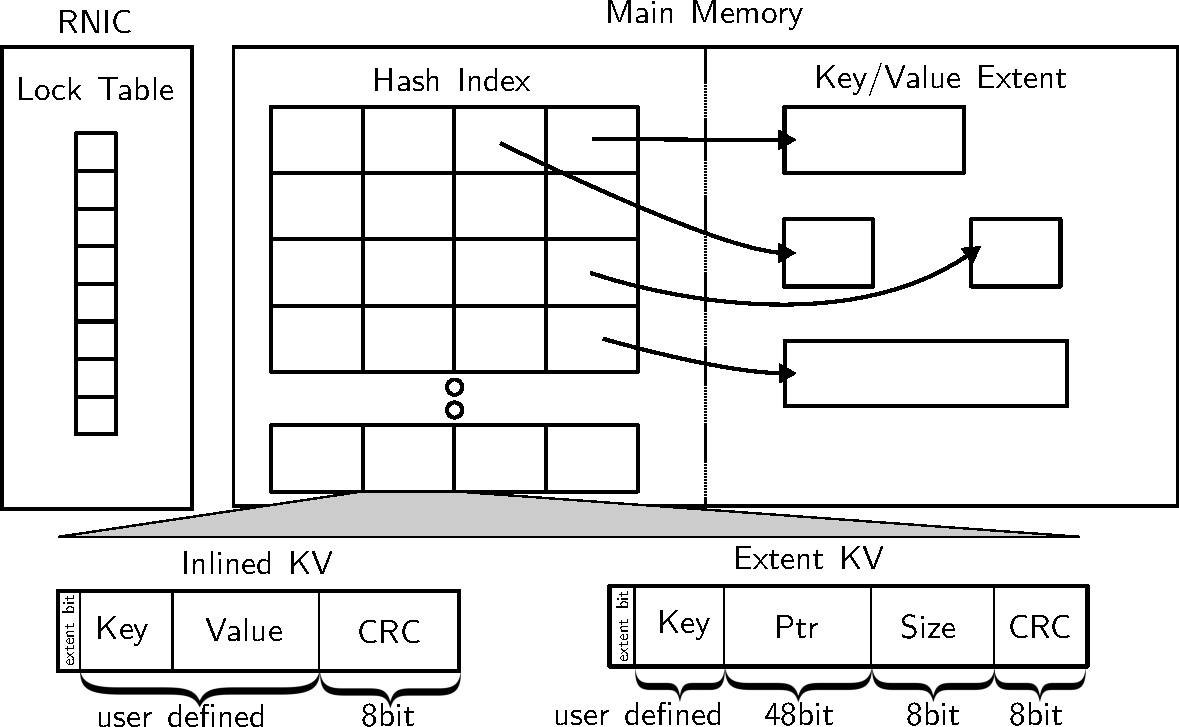
\includegraphics[width=0.99\linewidth]{fig/table-diagram.pdf}
    \caption{Rcuckoo's table design ~\todo{remove extents for this submission}}
    \label{fig:table-diagram}
\end{figure}


\subsection{Protocol}

\begin{figure}[t]
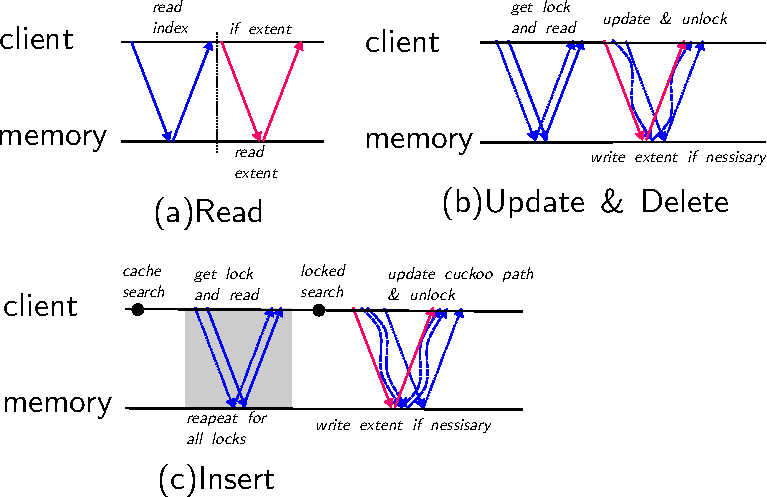
\includegraphics[width=0.99\linewidth]{fig/message_diagram.pdf}

\caption{Rcuckoo's protocol for reads, inserts, deletes and
updates. Blue lines are index accesses, and red lines are
extent accesses. Solid lines are reads, dotted lines are
CAS, and curved dashed lines are writes.}

\label{fig:message_diagram}
\end{figure}

In this section we describe our protocol for reading,
inserting, and performing updates and deletes to an rcuckoo
hash table. Figure~\ref{fig:message_diagram} visualizes our
protocol.

\subsubsection{Reading} All reads are performed locklessly.
If keys and values are inlined clients complete reads in a
single round trip, otherwise a second round trip is required
to resolve a pointer and read the extent. 
%%
~\footnote{This design requires exactly one pointer
resolution in expectation that future RDMA NICs may provide
pointer resolution reads as a primitive~\cite{prism}}
%%
The index is modified concurrently by writes, clients must
therefore validate their reads by computing a CRC post
read~\cite{pilaf,cell}.
%%
In the base case clients compute both hash locations for a
key and issue two bucket sized RDMA read requests to the
index. As an optimization clients can perform reads using a
single packet. We define a read threshold of 512 bytes for
our clients, if two hash locations are within 512 bytes we
issue a single large read.  Approximately 60\% of keys for
64-bit entries with a bucket size of 8 (see
Figure~\ref{fig:locality-hashing}(b)) fall into this
category. This has the advantage of updating the client
cache for future operations.
%, and reduces the header
%processing required by the NIC.
To reduce bandwidth the size
of the threshold can be tuned down, or turned off with no
harm to correctness.

\subsubsection{Locking and unlocking}

Update, delete and insertion operations all require locks to
modify the index. Locks are acquired in incremental order
from smallest to largest to avoid deadlocks. First the list
of locks required for the operation is calculated. For
updates and deletes two locks may be required. Inserts may
required many locks. The client calculates which locks it
requires and breaks the list into masked CAS operations
spanning 64 locks and then issued the requests polling for a
successful response before moving to the next lock.

To synchronize the client cache with remote memory we issue
a \textit{covering read}. A covering read is an RDMA read
which spans the range of buckets from the lowest lock in the
masked CAS to the highest. The covering read is issued after
the masked CAS and ensures the client receives synchronized
data for the locked buckets while not consuming an
additional round trip.

% Clients need their caches synchronized with remote memory
% prior to modifying it with writes. We batch reads with lock
% requests to synchronize client caches. RDMA in-order
% delivery ensures that reads issued after a lock request will
% be up to date, as no other client can concurrently modify
% the locked index.  A spanning read is issued for each lock
% request. The read covers each bucket the client locks.  For example, if a
% masked CAS has three locks, reads are calculated for each
% bucket being locked. If the locks cover a range less than
% the read threshold a single read is issued which spans all
% buckets between the locks.  Spanning reads are issued concurrently with
% lock requests.
%Subsequent lock requests are issued prior to
%blocking on reads.

After locks are acquired the client can execute its critical
section. Unlock requests are the inverse masked CAS operations of the
lock requests. Clients issue their critical sections as a sequence of
(asynchronous) writes followed immediately by unlock operations. RDMA
in-order delivery ensures that the unlock operations are performed
after the writes.

\subsubsection{Updates and Deletes}

Updates and deletes are performed in a similar fashion.
First the client acquires locks for both hash locations. If
the key is present the client issues the update or delete.
If the key is not present the delete fails, while the update
will then perform an insert, as described in the following
section. For updates the client updates the value and CRC of
the entry, on deletes the entry is set to NULL, and all
entries of the bucket are shuffled down to fill the hole.
%%
If extents are being used updates asynchronously write their
extent data during lock acquisition. Both updates and
deletes for extents remove the old extent data lazily.
Regardless of if extents are turned on updates and deletes
are performed in two round trips.

\subsubsection{Insert}

Unlike updates and deletes, inserts may require modifying
locations spread across remote memory and require many
locks. Determining which locks to aquire is hard as clients
may have stale caches and many options for potential
insertions paths.  We use a speculative two-phase search
strategy to find and execute insertions with high
probability in two rounds trips. First the client searches
it's local cache for a potential cuckoo path. Once a path is
found the client calculates the set of locks it requires and
attempts to aquire the locks for the speculative cuckoo
path. As locks are speculative reads synchronize the client
cache.

After the speculative locks are acquired the client performs
a second search only using the locked buckets in the table.
If no such path can be found, the client releases the locks
and tries again. If a new path can be found using the locked
buckets that path is executed and the lock is released.
This search strategy benefits greatly from course grained
locks. We have found in practice that setting each lock to
cover 8 buckets yields the highest performance. Given the
distribution of the locality hash function there is high
probability that an insertion path can be found within the
64 locked buckets. In the common case this means that
inserts take only two round trips. On failures the client
maintains the cache it built during the first search to
improve its chances of finding a path on the next attempt.


% We use a two-phase search
% strategy to find insertion paths. First the client
% constructs a potential cuckoo path using its cached index.
% The client then attempts to acquire the locks necessary for
% its cuckoo path. Thanks to the spanning reads, once a client
% succeeds in acquring the necessary locks its cache has been
% fully synchronized with the relevant portions of remote
% memory. A second search is then performed using only the
% buckets the client succeeded in locking---which may be the
% same if the client's cache was completely up to date. If
% this search is successful the client calculates the updates
% to the cuckoo path batches them as a series of writes and
% issues them along with it's unlock requests.

% If the first search fails the client performs a read and
% tries again. If this fails the table must be resized. The
% second search may fail because the clients cache was stale
% and the list of locked buckets was insufficient to perform
% the insert. In this case the client releases the locks and
% performs the insertion from the start again by performing an
% unrestricted search on its local cache. In the common case
% insertions take two round trips: We find that when the table is less
% than 50\% full the probability that a cuckoo path has
% length greater than one is low. If extents are
% used the client batches the extent write during its locking
% phase.

% \textbf{Key Duplication:} Unlike RACE our algorithm can
% prevent duplicate keys easily on insert~\cite{race}. RACE
% requires three round trips for inserts, the third re-reads
% the index to ensure no duplicates were inserted
% concurrently.  Alternatively Cuckoo hashing inserts to
% exactly one bucket, which is read during the lock
% acquisition phase. If a duplicate key is found the client
% can abort. If the bucket is full, a duplicate key may exist
% in itts alternative bucket. Our clients issue a read to the
% inserted keys alternative bucket during lock acquisition. If
% the lock returns successfully and no duplicate exists in
% either bucket then no duplicates exist as the successful
% lock ensures that no other client is currently moving the
% key to another location as part of a concurrent insert.


\subsubsection{A* Search} 

Locality based hashing provides us opportunities for better
search than traditional cuckoo hashing. Cuckoo hashing
insert traditionally uses random replacement~\cite{cuckoo}.
Random replacement requires little computation, however at
high fill rates it leads to long cuckoo paths which require
many locks, and reduce concurrent throughput. BFS search
finds the shortest path and has been demonstrated to
increase system throughput with fine-grained
locking~\cite{cuckoo-improvements}.  BFS is computationally
intensive. Locality based hashing enables us to leverage
more efficient search strategies. Because locality hashing
increases the probability that a cuckoo hashing location is
close we can use an informed search algorithm to find open
slots close to bucket a key hashes to. 
%%
In the case of BFS the target bucket is unknown, therefore
all paths must be explored. We use A* search, an algorithm
which takes a goal location, and a distance heuristic as
input. A* is known to find shortest paths in much better
average-case times than BFS~\cite{}. A* requires two
additional inputs, a distance heuristic and a goal location.

\textbf{Goal location}: Locality hashing increases the
probability that an open slot near the insertion target
location can terminate a cuckoo path. Our algorithm collects
open slots near the original hash location as candidate goal
locations. By default we set the number of candidate goal
locations to 5. Goal locations are collected by starting at
the $h_1(k)$ location and iterating through the hash
table both forward and backwards through the table one index
at a time. Buckets with open slots are added to the
candidate list until the limit is reached. 

% \todo{I could
% improve this search time by tracking the list of open
% buckets and using binary search on them.}.

\textbf{Search Heuristic}: A* requires a heuristic for
distance which is a strict underestimate of the true
distance to a goal. A typical heuristic for search is the
euclidean distance between two points. A * guarantees that
if the search heuristic is a strict underestimate of the
true distance to the goal then the path found will be the
shortest path. In our case we use the distance between a
goal state and a current state is unknown as the distance
between any two buckets is the result of our locality
hashing function which has no upper bound. However we can
estimate the distance between two buckets by using the mean
distance of our locality hash function. This approach does
not guarantee that we find the shortest path, however it
does find short paths in the common case, and results in
very short search times.